%Observação importante: para usar os recursos da classe ABNTEX, é necessário fazer o download de sua biblioteca,
%visto que a mesma não é nativa do ambiente \LaTeX.
%Em um distribuição linux baseada em debian o pacote pode ser instalado pelo comando: sudo apt-get install abntex.
%Autor:Jean Henrique Ferreira Freire

\documentclass{abnt}
\usepackage[brazil]{babel}
\usepackage[utf8]{inputenc}
\usepackage[num]{abntcite}
\usepackage{graphicx}
\usepackage{amsthm}
\usepackage{url}

\begin{document}
\autor{Vitor Botelho Vaz de Melo}

\titulo{Identificando Linhas de Códigos Comentadas em Repositórios de Software}

\orientador[Orientador:\\]{André Hora - Departamento de Ciência da Computação}




\comentario{Proposta de Projeto de Pesquisa e Tecnológico da disciplina de Projeto Orientado em Computação do DCC/UFMG}

\instituicao{Universidade Federal de Minas Gerais \par Instituto de Ciências
Exatas \par Departamento de Ciência da Computação}

\local{Belo Horizonte} \data{2019/1}

% \capa 

\folhaderosto 


% \begin{resumo}
% Coloque aqui seu resumo.\\


% \textbf{Palavras-chaves}: palavras, chave. 
% \end{resumo}

% \sumario %comando que gera o sumário automaticamente
% \renewcommand*\listfigurename{LISTA DE FIGURAS}
% \listoffigures %comando que gera um sumário para a lista de figuras do texto automaticamente



\chapter{INTRODUÇÃO}


À medida que a Ciência da Computação avança e milhões de linhas de códigos são 
escritas, diariamente e em diversas linguagens de programação, os desenvolvedores 
percebem que, para alcançar sucesso a médio e longo prazo em seus projetos, é
necessário utilizar-se, cada vez mais, das melhores ferramentas e práticas de 
programação. 

Uma prática de programação muito comum ao se desenvolver softwares é a de 
''remover'' uma linha ou um bloco de código tornando-os comentários, sendo conhecida  
como commented-out code (Figura \ref{fig:commentExample}). Comentar uma linha de código 
pode ser útil, tanto que 
os próprios ambientes de programação (IDE's e editores de texto) oferecem atalhos 
fáceis para isso. Contudo, esta prática se torna um verdadeiro problema quando 
estes códigos comentados estão inseridos em um sistema grande, complexo e
mantido por diversas pessoas.\cite{cleanCode}.

\begin{figure}[h!]
  \centering
  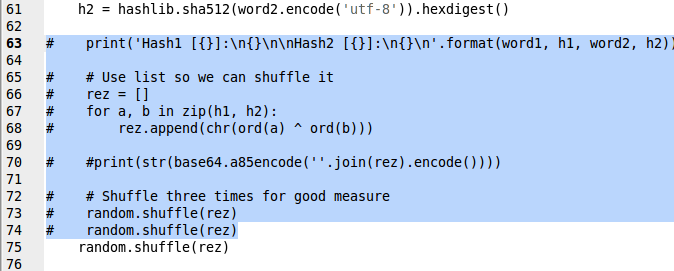
\includegraphics[height=2.4in,width=6.3in]{images/gcc06.png}
  \caption{Commented-out code example }
  \label{fig:commentExample}
\end{figure}


A inserção de código comentado nos arquivos fontes de um sistema pode causar
redução da legibilidade, distração e perda de tempo. Martin, em seu livro clássico
Clean Code, enfatiza \textit{Few practices are as odious as commenting-out code. 
Don’t do this!}, ele argumenta que outras pessoas não terão coragem de deletar 
este código por achar que ele pode ser importante~\cite{cleanCode}. 

Além disso, quando um mantenedor se depara com códigos comentados ele pode ter uma 
série de dúvidas, como \textit{"Por que este código está comentado? Isso é útil em 
alguma função? Este código está relacionado com determinada mudança?"}, entre outras 
questões específicas para cada sistema. Este tipo de reflexão pode no mínimo ser 
uma perda de tempo, ou até mesmo uma distração para introduzir bugs no sistema \cite{cleanCode}.

Este trabalho tem como principal objetivo fazer um estudo abrangente desta prática em repositórios 
de código aberto. No entanto, existem poucos estudos científicos abordando esta problemática e não 
há, entre as ferramentas mais populares, uma solução que identifica automaticamente
este tipo de comentário \cite{articleMiningComments}. Portanto, na disciplina Projeto Orientado
em Computação I, será desenvolvido uma ferramenta apropriada utilizando técnicas de aprendizado de 
máquina e, a partir disso, na disciplina Projeto Orientado em Computação II, será realizada a análise de
diversos sistemas. 


\chapter{REFERENCIAL TEÓRICO}


\section{Trabalhos Anteriores}

GRIJÓ L. e HORA A. exploraram o problema da inserção de código comentado 
e demostraram interessantes resultados no artigo Minerando Código Comentado 
\cite{articleMiningComments}. No trabalho foi desenvolvido um parser heurístico
que identifica \textit{commented-out code} para a linguagem java que, e obteve
uma precisão de 83\%. Com esta ferramenta foi identificado que alguns 
sistemas possuem como mediana 4,17\% de taxa de commented-out code em relação
ao total de comentários, com alguns sistemas chegando a 30\%.

Neste trabalho é proposto uma metodologia multi-linguagem baseada em técnicas de
aprendizado de máquina. Tem se a ambição de superar a precisão da ferramenta
desenvolvida no trabalho anterior, possibilitando a validação dos resultados 
encontrados e generalizá-lo para diversas linguagens.


\section{Mineração de Repositórios de Software}

Para se entender as práticas e diversas informações sobre um sistema pode-se
analisar as diferentes versões do código deste sistema. Dessa forma pode-se 
identificar em um sistema as boas e más práticas presentes, questões arquiteturais,
entre outras questões, com o objetivo de melhorar a manutenibilidade deste sistema.
Através da mineração de repositório de software podemos 
predizer quais seções do código apresentam mais defeitos e maior
dificuldade de compreensão; usar a evolução do software para identificar
partes do código que são mais importantes para manutenção; entender como diversos
desenvolvedores e times afetam a qualidade do código.
\cite{crimeScene}. 


\section{Git e GitHub}

Git\footnote{https://git-scm.com/} é uma ferramenta amplamente usada na 
comunidade de desenvolvimento de software para controle de versão de código.
Ela permite que seja avaliado diferentes versões do código de um mesmo 
sistema~\cite{articleMiningGit}. O Github\footnote{https://github.com/} é 
uma plataforma que permite hospedar repositórios de código com o sistema de versionamento
Git na nuvem. Nele é possível encontrar diversos repositórios de código aberto 
que serão as fontes de estudo deste trabalho. 

\section{Algoritmos de Classificação}
Os algoritmos de classificação são algoritmos de aprendizado supervisionado,
no qual utilizamos uma base de treino em que previamente sabemos a "classe" 
de cada objeto para treinar um modelo que pode dizer qual a classe dos 
objetos dos quais não conhecemos \cite{patternClassification}.

Podemos modelar o problema de identificar \textit{commented-out code} como sendo um problema
de classificação binária. Neste caso, os objetos serão os comentários presentes em 
códigos de diversas linguagens, e a classe será se aquele comentário é normal 
representado por 0 ou código comentado representado por 1.

\subsection{Precisão e Revocação}
As taxas de precisão (\textit{precision}) e revocação (\textit{recall}) nos permite avaliar a qualidade do classificador~\cite{powers2011evaluation}.
Elas são definidas como:
\begin{center}
  

\begin{math}
  precision = \frac{tp}{tp +fp}
\end{math}~~~~~
\begin{math}
  recall = \frac{tp}{tp +fn}
\end{math}
\end{center}

\begin{itemize}
  \item tp = True Positive: Elementos classificados como 1 ou positivos corretamente.
  \item fp = False Positives: Elementos classificados como 1 ou positivos incorretamente.
  \item fn = False Negative: Elementos classificados como 0 ou negativos incorretamente.
\end{itemize}


\chapter{METODOLOGIA}

\section{Extração e Preparação dos dados}

Os comentários deverão ser extraídos de diferentes repositórios de software. 
Em sequência, estes comentários deverão ser classificados manualmente
como \textit{commented-out code} ou comentário normal a fim de se formar 
a base de treinamento. Esta base deverá contemplar diferentes tipos
de linguagem para que o classificador consiga identificar códigos
comentados independente de linguagem. Dessa forma teremos uma base de dados em que o 
X será igual a uma linha de comentário e o Y igual a 0 se for um comentário 
normal ou 1 se for um código comentado, que servirão, respectivamente, como input 
e output para o treinamento do classificador.

\section{Treinamento de Modelos de Classificação}

\begin{figure}[h!]
  \centering
  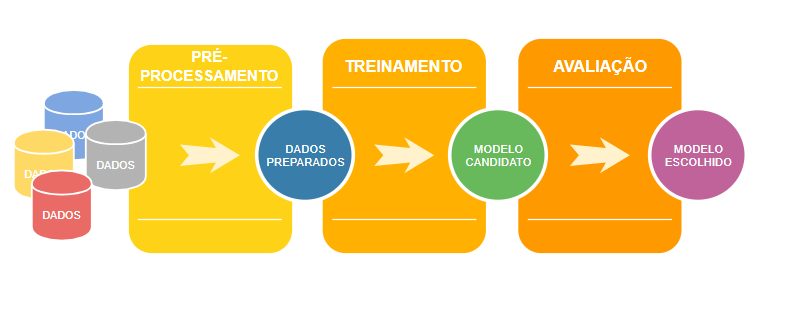
\includegraphics[height=2.4in,width=6.3in]{images/processing.png}
  \caption{ Procedimento básico para definição do modelo de classificação}
  
  \label{fig:fluxo}
\end{figure}

A figura \ref{fig:fluxo}  ilustra os passos básicos para encontrar um modelo de classificação
\footnote{Exemplo extraído de https://gabrielschade.github.io/2018/01/08/machine-learning-intro.html}.
Primeiramente, a partir dos dados coletados e classificados, devemos pré-processar
os textos de comentários para que possam ser \textit{inputs} do modelo.
Pretende-se usar uma representação binária, baseada em caracteres, que será
melhor definida ao longo do trabalho.
Em sequência, será selecionada uma variedade de modelos/algoritmos de classificação,
como, por exemplo, redes neurais multi-layer perceptron~\cite{zurada1992introduction}
~\cite{patternClassification}, LSTM~\cite{gers1999learning} , dentre outros. 
Por fim, será computado os índices de precisão e revocação dos modelos para se definir
o melhor modelo.




\section{Compilação de dados de Repositórios}

Com a ferramenta de identificação de códigos comentados preparada, serão analisados 
diversos repositórios relevantes de softwares de código aberto, encontrados
no GitHub. Ao identificar os comentários, será possível calcular a taxa de 
código comentado em relação ao total de comentários em uma versão do 
software, e com o auxilio da ferramenta Git será analisado a evolução do 
software através do código em diferentes versões. Com isso teremos 
indícios de como os desenvolvedores estão lidando com essa prática, entre 
diversas outras informações que podem ser exploradas com este tipo
de técnica.

\chapter{RESULTADOS ESPERADOS}

Espera-se que ao final da disciplina Projeto Orientado em Computação I  
obtenha-se uma ferramenta robusta e com alto nível de precisão para identificar 
códigos comentados em diversas linguagens de programação. No final da 
disciplina Projeto Orientado em Computação II espera-se compreender como a 
má prática de remover código através de comentário afeta a evolução dos 
diferentes repositórios de código aberto, respondendo perguntas como:
\textbf{(1)} Qual a taxa de código comentado média nos repositórios de software?
\textbf{(2)} Como essa taxa evolui ao longo das versões.
\textbf{(3)} Ela varia dependendo da linguagem?
\textbf{(4)} Existe uma correlação entre arquivos mais modificados e a presença de 
    código comentado?,
dentre outras questões.



\chapter{ETAPAS E CRONOGRAMAS}

\begin{table}[ht]
  \centering
  \label{tab:Table1}
  \smallskip
  \begin{tabular}{cp{11cm}}
  Período & Atividade\\[0.5ex]
  \hline
  19/03 a 12/04 & Estudo e elaboração da proposta do projeto. \\[0.5ex]

  13/04 a 28/04 & Criação de uma ferramenta para extração dos comentários em 
  repositórios de software abertos.\\[0.5ex]
  
  29/04 a 19/05 & Classificação dos dados extraídos para definição da base 
  treino. Elaboração e Apresentação intermediária. \\[0.5ex]

  20/05 a 16/06 & Treinamento e avaliação de um modelo de classificação para 
  identificação de \textit{commented-out code}. \\[0.5ex]

  17/06 a 05/07 & Elaboração do artigo, poster e apresentação final. Submissão 
  do artigo científico com os resultados parciais para o evento VEM 
  (Workshop on Software Visualization, Evolution and Maintenance) \\[0.5ex]
  \end{tabular}
  \end{table}

  Na disciplina de Projeto Orientado em Computação II será desenvolvido
  o restante das atividades, sendo elas: seleção e extração dos repositórios 
  a serem avaliados, definição de métricas relativas a \textit{commented-out code},
  desenvolvimento de uma ferramenta para computar, salvar e visualizar os 
  resultados encontrados.


\bibliography{references.bib}

\end{document}
